\chapter{Method}
As mentioned in chapter \ref{SoA},human attention is defined such that we have two approaches which are bottom up and top down. 
In this chapter we first explain our main tool and our choices.
Then we are going to focus on the bottom up approach, using eye tracking data captured while chess player were playing games, training our network only on this data. Features are extracted and the network is learning how to produce visual attention map from them. 
Finally we will discuss how we started to think about the top down approach, which is leading visual attention based on the action we have to do. The conclusion being a quick overview of our implementation.


\section{Attention prediction Network and dataset}\label{section:model}
\begin{figure}[h!]
 \centerline{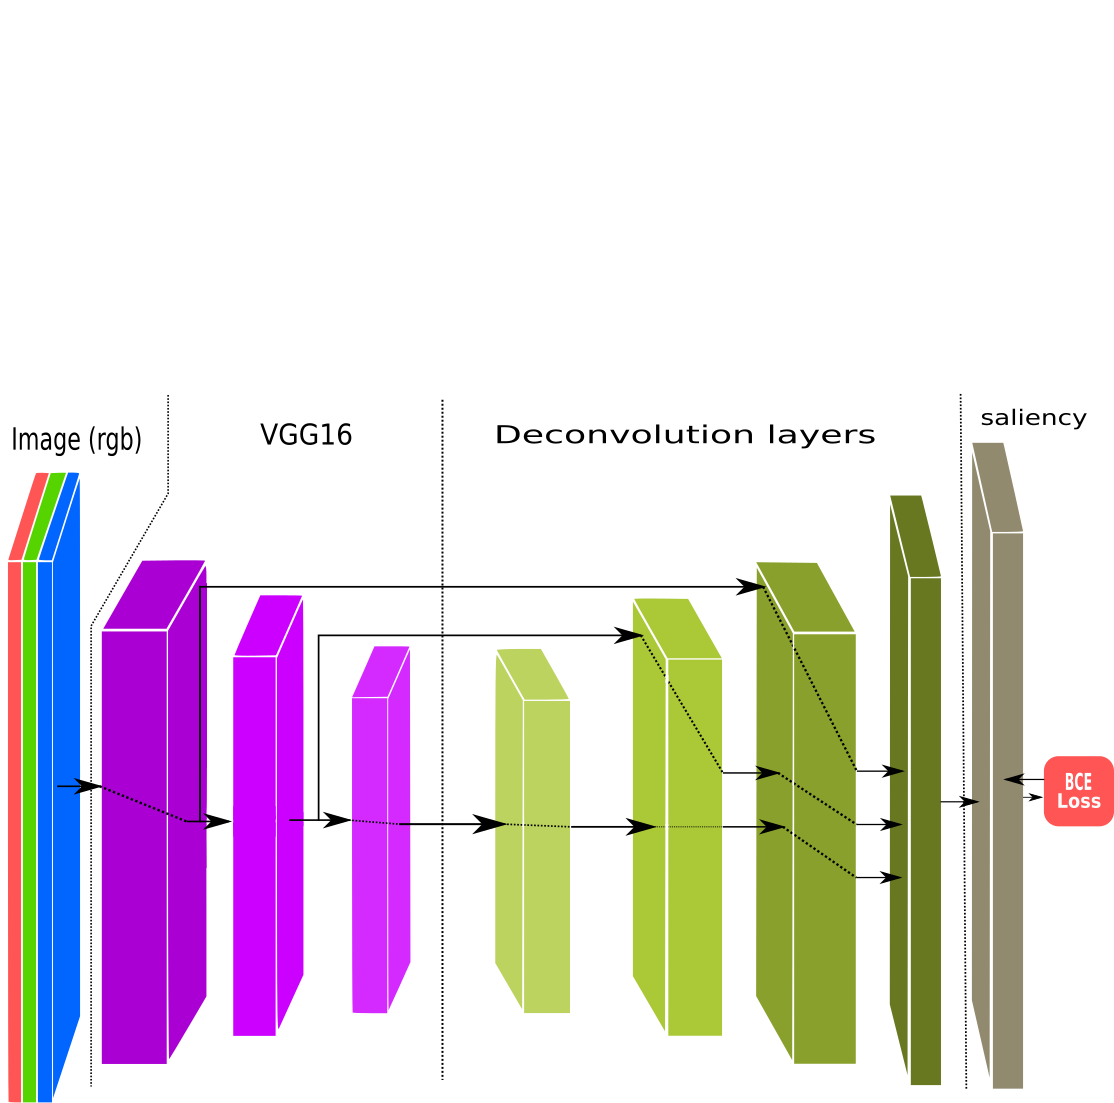
\includegraphics[scale=0.40]{./pics/network.png}}
 \caption{Our network}
 \label{fig:network}
\end{figure}
Our model presented in figure \ref{fig:network}, is inspired by the one used in Wang, and al. paper \cite{DBLP:journals/corr/WangS17b}. We use a multi-scale approach based on the skip-layer architecture, common in attention prediction. The first part (encoder) is the VGG16 \cite{DBLP:journals/corr/SimonyanZ14a} architecture, while the second part (decoder) is a succession of deconvolution layers stacked one on top of the others. The difference between our model and \cite{DBLP:journals/corr/WangS17b}, is that we share weights between these deconvolution layers. Their weights are initialized using a normal distribution, with a mean of 0 and a standard deviation of 0.01.


Sharing weights has several advantages. The first obvious one is the size of memory for deconvolution weights reduced by 5 in this case. The number of parameters to optimize is also reduced and thus the network is converging way faster.
We had also an other intuition behind sharing weights. Because we take features at different scale in the Encoder part of the network, outputs of those layers have different field of view. At a small scale, with a reduced field of view,let say of maximum 2 cells. If we have a bishop endangered by a pawn, translated as a local feature map, it is logical that this relation become salient in the final saliency map. Now if we take the same relation between the two pieces, but this time across the board, where the bishop can take the enemy pawn, the network should consider this to be salient the same way as before but at a larger scale/field of view. This is why a feature map, upsampled using deconvolution, should be deconvoluted using the same weights as an other feature map of the same dimensions.


The input of the network is a image encoded on three channels (Red, Green and Blue), resized to 224 pixels by 224 using bilinear interpolation. We could use inputs encoded on the gray scale only. However our network is based on transferring knowledge from previously trained VGG network \cite{DBLP:journals/corr/SimonyanZ14a}. This previous knowledge was acquired using features from colored images. We show in section \ref{section:pretrain}, how this knowledge transfer is important and thus why we keep an input encoded on three channels. The last layer of the network which is producing a saliency map of the size of the input image, is doing the following :
\begin{itemize}
    \item Crop the three outputs from the last convolution to the size of the input image (output shape :[3,224,224]) 
    \item Repeat them three times and stack them up (output shape : [9,224,224])
    \item Execute a final deconvolution on this stacked up data, to output a tensor of the shape [1,224,224]
    \item A Sigmoid function is applied on it to map the saliency values between 0 and 1.
\end{itemize}

All those steps end up giving us a saliency map, the same size of the original picture, encoded between 0 and 1.

\subsection{Deep learning layers}\label{Deep learning}

In this section we are going to describe few layers and methods we use in our model. Our model being based on convolution, we explain why using them and their principal components(Padding and stride) in section \ref{section:conv}. We then explain their counter parts name "deconvolution" and the pooling method. Finally we give a brief overview of Transfer learning and why using it in section \ref{section:transfl}.


\subsubsection{Spatial convolution}\label{section:conv}

Using a regular network such as a perceptron which is using only linear operations and activation function won't be a good idea when considering images. For example if we take a 300x300 rgb picture, we would need 2700001 parameters for a single neuron making the memory size of a network exploding. But images have spatial relationships which we can take advantage of, by convolving a set of N filters on the images creating  N 2D feature maps. Spatial convolutions are defined by the number of filter and the properties of the convolution (ie. padding and strides). \\

\textbf{Padding}\\

Padding is used to preserve information between convolutional layers and  the dimension of the output. Let say, we apply a 5*5 filter on a 32*32 input with a stride of 1, we would get an output of size 28*28, losing some information and quickly reducing the dimensions after few layers of convolution. For that we had some padding around the input to augment its dimension to 36*36,so that after the convolution layer the output keep the 32*32 dimension. Padding is simply adding some 0 values around the input. To keep the same dimensions with as stride of 1 the size of the padding is $p = \frac{k-1}{2}$ where k is the kernel size.\\

\textbf{Strides}\\

Strides control how we convolve the filter on the input. With a stride of 1 we move the center of 1 cell at a time, for a stride of 2, 2 cells at a time etc.. It allows to control the receptive field and how it overlaps.\\

\begin{figure}[ht!]
   \centerline{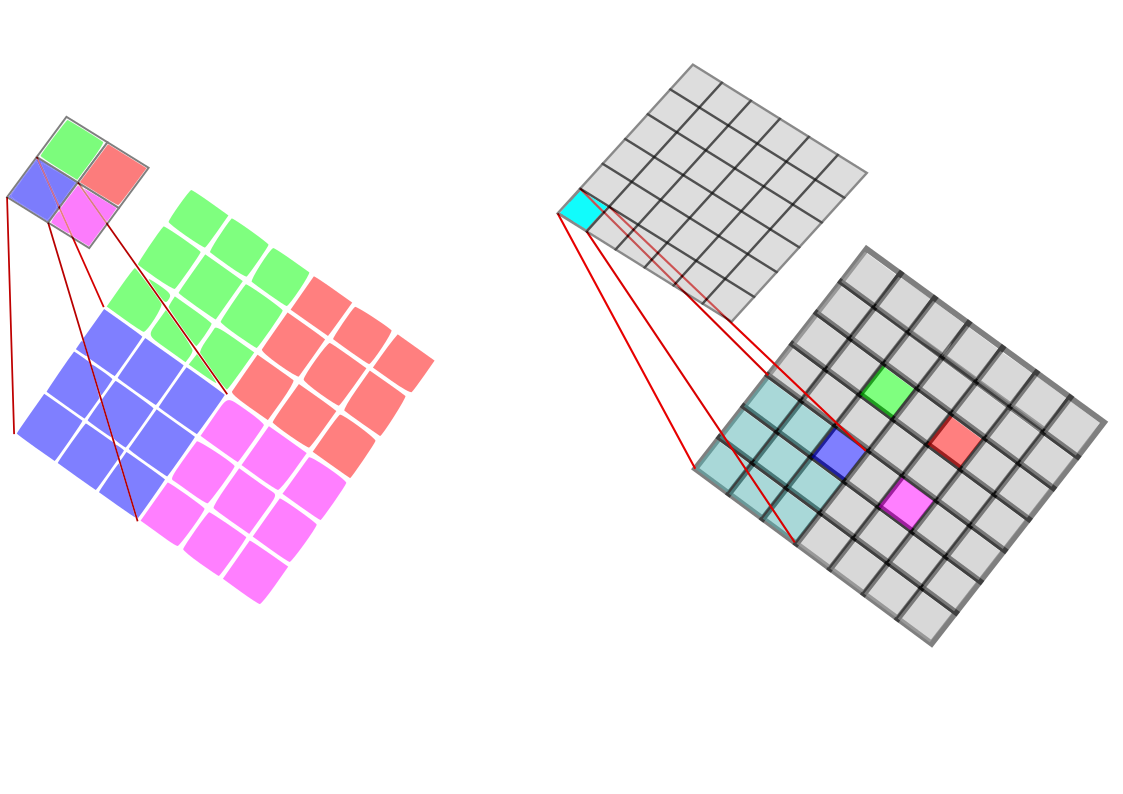
\includegraphics[scale=0.30]{./pics/convolution.png}}
   \caption{A convolution and its transposed counterpart}
   \label{fig:conv}
\end{figure}


The operation inverse to a convolution is a deconvolution, which is just basically reverting the operation done by a convolution.
In deep learning, deconvolution are not used but instead we use the Transposed Convolutions or fractionally strided convolutions which are wrongly called deconvolution. A deconvolution of an input 2*2 should get 9 values out of one for a previous convolution of a kernel of size 3 with a stride of 2. But because this would be a bit tricky, we instead do a simple convolution over the input, using some padding on it. The figure \ref{fig:conv} shows how a convolution is applied on an input and how the transposed convolution is computed on the result. The left part is the convolution applied on the 6*6 picture with 0 padding and stride of 2. The right part is how the transposed convolution is computed to get back to the original picture. A padding of two is added around the input and 0 values are inserted between the input values (because of the stride of 2).


\subsubsection{Pooling}

Pooling is used to reduce the size of the feature map by aggregating multiple cells in a single one, it also produce invariance to small variation between images. Several way of pooling exist such  as \textbf{Maxpooling} which is taking the maximum of the values in the area of the size of a filter, or \textbf{AveragePooling} taking the average instead. Figure \ref{}  illustrate pooling over a feature map.


\subsubsection{Transfer learning}\label{section:transfl}

Transfer learning start from the idea that features learned from huge amount of data, are relatively the same when looking at the first layers of Deep neural networks. Thus it if often not useful to retrain from scratch our network while we could start from already trained weights which can be pretty close to what the final weight of our network would be on our specific dataset. 
In their survey paper \cite{Pan:2010:STL:1850483.1850545}, Pan an al., worked on categorizing, explaining and discussing advancement on transfer learning up until 2009. Offering a broad explanation on techniques and work done on this part of the deep learning field.


\subsection{Data pre-processing}
The data given as an input to our network does not need a lot of pre-processing other than being re-sized and cropped to be just the size of a chess board. On the other hand some work needed to be done on the ground truth data being heatmaps from eye tracking data. The heatmaps were produced by an eye tracking software (Tobii Studio 3.4.7) which was simply doing a convolution of colored Gaussian on user's fixations. The problem was that the color scheme use for those Gaussian was not directly transformable to grey scale data by taking the average of the three channels Red Blue and Green. Figure \ref{fig:gray} Shows a heatmap taken from the eye tracking software and converted to grayscale.\\

\begin{figure}[ht!]
    \centering
    \begin{tabular}{c@{\hspace{0.2cm}}c@{\hspace{0.2cm}}c@{\hspace{0.2cm}}c}
    
        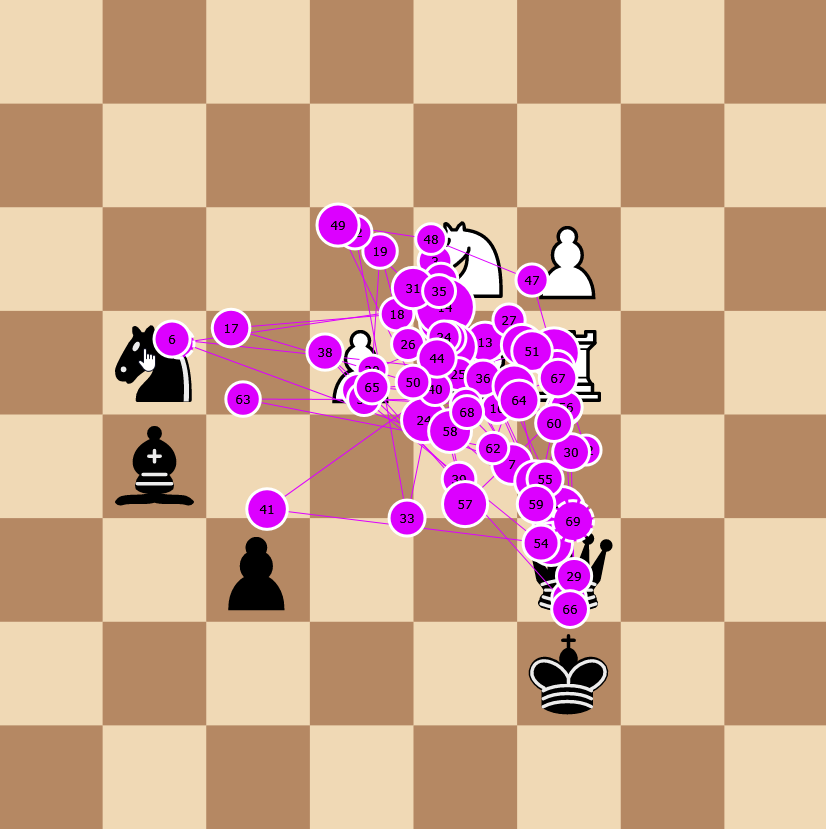
\includegraphics[width=0.25\linewidth]{./transformations/origin.png}& 
        
\includegraphics[width=0.25\linewidth]{./pics/base_image.png}& 
        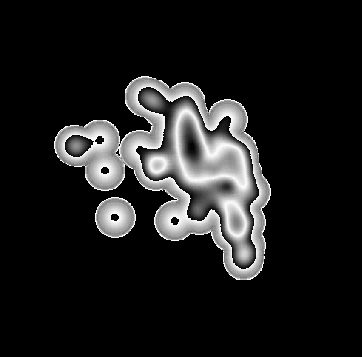
\includegraphics[width=0.25\linewidth]{./pics/color_to_gray_wrong.png} & 
        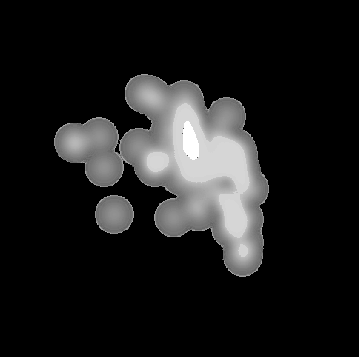
\includegraphics[scale=0.313]{./pics/correct_gray.png}\\
        {\small  Scan path} &{\small  Heatmap} & {\small Gray scale conversion (A) } & {\small A correct representation (B)}\\ 
        {\small  } & {\small  } & {\small  by averaging} & {\small of gray scale}\\ 
         {\small  } &{\small  } & {\small  } & {\small }\\ 
    \end{tabular}
    \caption{From scanpath to heatmap to incorrect gray scale representation (A), and correct gray scale representation (B)}
    \label{fig:gray}
\end{figure}
The solution was to create ourselves the translation from Red Blue and Green encoding to a gray gradient between 0 and 1. Red (encoded as [255,0,0]) became 1, decreasing through orange  ([255,>128,0]) and yellow ([255,255,0]), to light green ([0,255,0]) and darker Green ([0,>150,>50]. Taking in consideration the value of Green for closer to red colors and Blue for color closer to green, allowed us to create a gradient representation as in figure \ref{fig:gray} (contours of Gaussians being brighter than the inside is due to a bug from the eye tracking software, which is adding lighter green to the exterior of  Gaussians).

Our model is close to a standard auto-encoder architecture which basically learns to encode some data and to decode it to be like the input. The logic way to compare its output to the input would be to compute the distance between them and to minimize it. 
For that there is the basic, simple and intuitive L1 loss, being $|y - f(x)|$ (with y as the GroundTruth and f(x) the output of the auto-encoder), could be a solution. We also have the L2 loss, also known as Mean square error express as $ (y- f(x))^2$.

But in our case we don't learn how to generate a copy of our input being a chessboard with pieces on it, but the visual prediction of this chessboard. The visual prediction is a probability distribution between 0 and 1, 0 being not looked at at all (black) and 1 long fixations (white) (or salient or not salient).
In statistics the Kullback Leibler divergence \cite{10.2307/2236703} express how much two probability distributions are diverging one from the other, minimizing it is equivalent to reducing the distance between them. 
It can be expressed as the equation \ref{eq:KL}.
\begin{equation}
    \label{eq:KL}
    KL(P|Q) = \sum\limits_{i=1}^n P(i) \frac{P(i)}{Q(i)}
\end{equation}
However Kullback Leibler divergence is not a metric as it doesn't respect the triangle inequality and often $KL(P|Q) \neq KL(Q|P)$. But if we develop the expression of equation \ref{eq:KL} in \ref{eq:devKL}:

\begin{align}
\label{eq:devKL}
KL(P|Q) & = & \sum\limits_{i=1}^n P(i) \frac{P(i|x)}{Q(i|x)}\\  
& = & \sum\limits_{i=1}^n ( - P(i|x) log(Q(i|x))  + P(i|x) loq(P(i|x)))\\
& = & - \sum\limits_{i=1}^n   P(i|x) log(Q(i))  + \sum\limits_{i=1}^n P(i|x) loq(P(i|x))\\
& = &  -\sum\limits_{i=1}^n  P(i|x) log(Q(i|x)) - \sum\limits_{i=1}^n P(i|x) loq(\frac{1}{P(i|x)})\\
&  = & -\sum\limits_{i=1}^n   P(i|x) log(Q(i|x)) - H(P(i|x))
\end{align}

If we take our Ground truth as P, because it doesn't change its entropy is equal to 0 and we have just the cross entropy between our two probability distributions $ -\sum\limits_{i=1}^n   P(i) log(Q(i)) $
Taking a binary approach, with i being either 0 or 1 (salient or not salient), $Q(i|x) = y$ our Ground-truth  and $P(t|x) = c$ the output of our model, we can write $-\sum\limits_{i=1}^n   P(i|x) log(Q(i|x)) - H(P(i|x)) = -ylog(c) - (1-y)log(1-c) $, giving us the formula of the Binary Cross entropy. 
We show that binary cross entropy in the case of saliency map generation can be seen as relatively close related to the Kullback Leibler divergence. Minimizing it would allow us to generate data as close as possible to the groundtruth.

Also we will no use Kullback Leibler divergence as a metric in this report for several reasons discussed in \cite{LeMeur2013} and \cite{metricsreview} among other paper cited in this report. The first one being that this distance is non-linear, non-symetric and it doesn't respect the triangle inequality. Also the fact that there is no upper bound clearly defined is a problem. This distance between two generated saliency maps and a groundtruth, gives us an overall dissimilarity and allows us to see which one of the saliency maps has the highest.

\subsection{Dataset}
\subsubsection{Available data} \label{section:data}
The data we started with comes from the experiments of Thomas Guntz \cite{thomasguntz}. He worked on the multimodal study of people solving various problems and in particular chess problems. For his experiments he recorded the eye-gaze of several players from various level, trying to solve different chess task of increasing difficulty (from openings to king in check in N moves). There were 11 configurations (Figure \ref{fig:dataset}) on which  were captured around thirty players eye tracking data. Because visual attention is quite subjective and even if it depends on the chess player level, it often has some divergences. For that we decided to group all our heat-maps into one saliency map, being the average of them. Why the average? Because we didn't have the  same amount of people in the "expert" category than in the "amateur" one. Hence areas where the expert would focus wouldn't have been a good representation of the areas player often looks at. Averaging all those heat-maps we get a good idea of areas which are important for most of the players, those being less important are darker in the gray scale.

 \begin{figure}[ht!]
    \centering
    \begin{tabular}{@{}c@{\hspace{0.2cm}}c@{\hspace{0.2cm}}c@{\hspace{0.2cm}}c@{}}
        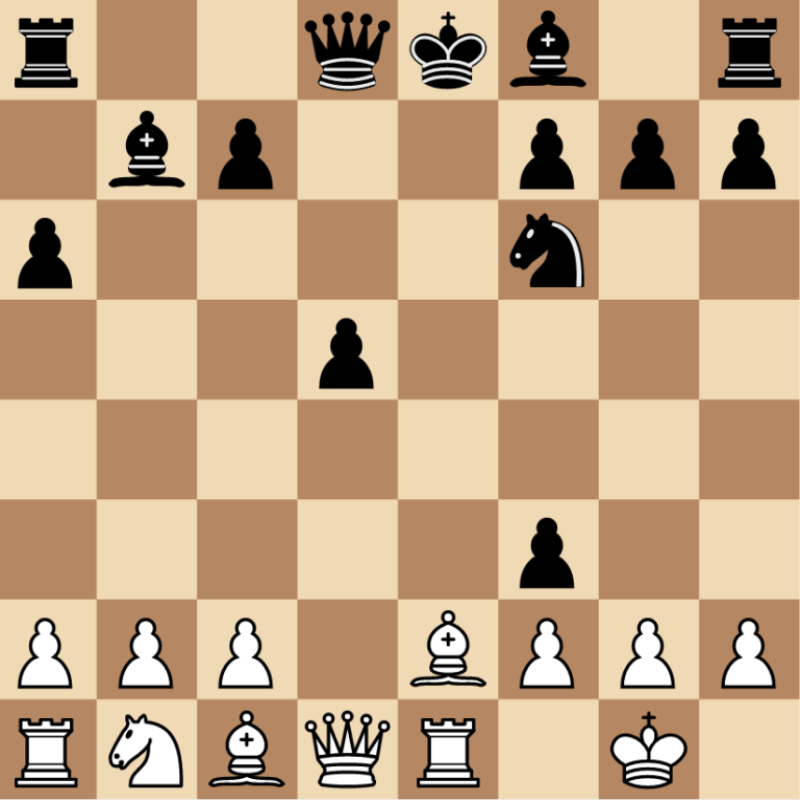
\includegraphics[width=0.25\linewidth]{./dataset/configIV.png}&
        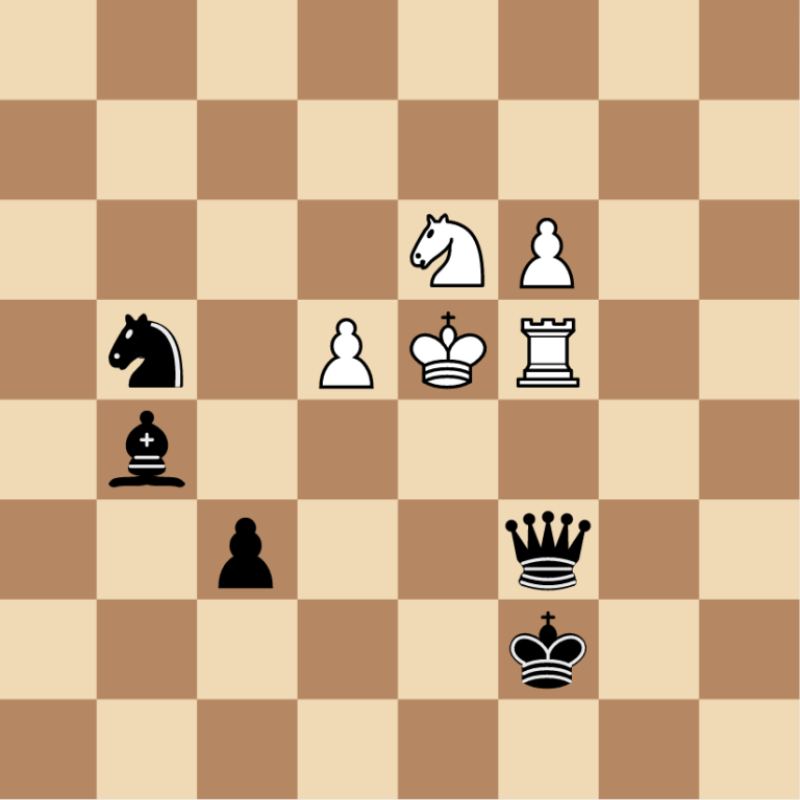
\includegraphics[width=0.25\linewidth]{./dataset/configIX.png}&
        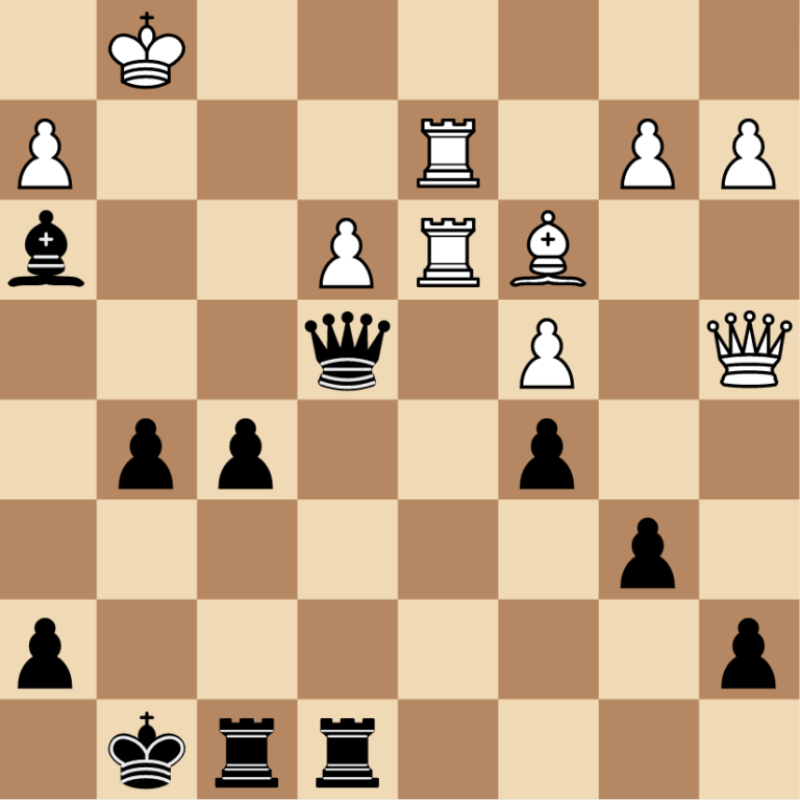
\includegraphics[width=0.25\linewidth]{./dataset/configLI.png}&
        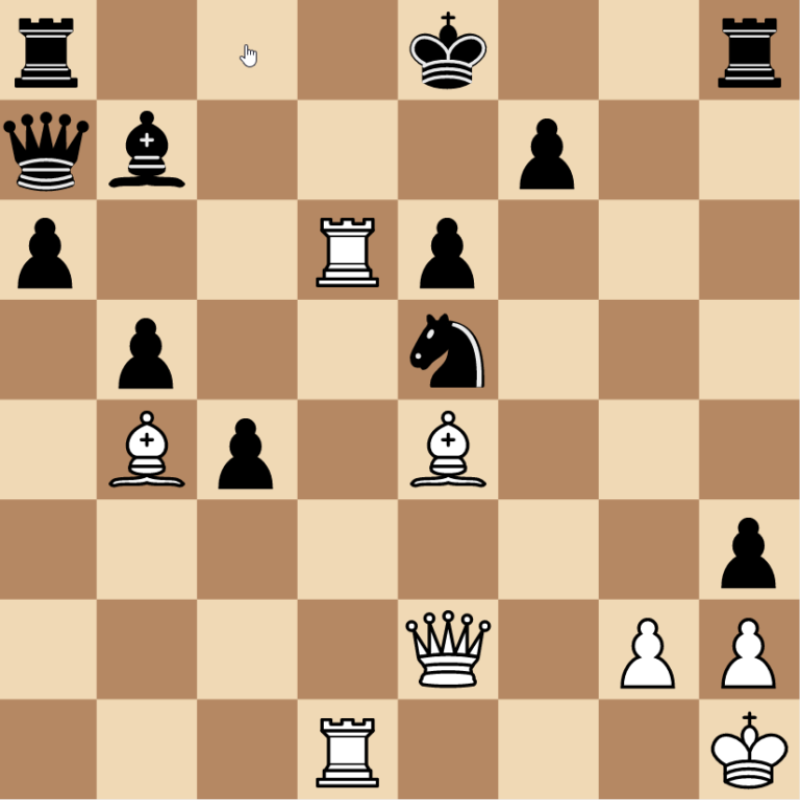
\includegraphics[width=0.25\linewidth]{./dataset/configLIX.png}\\
        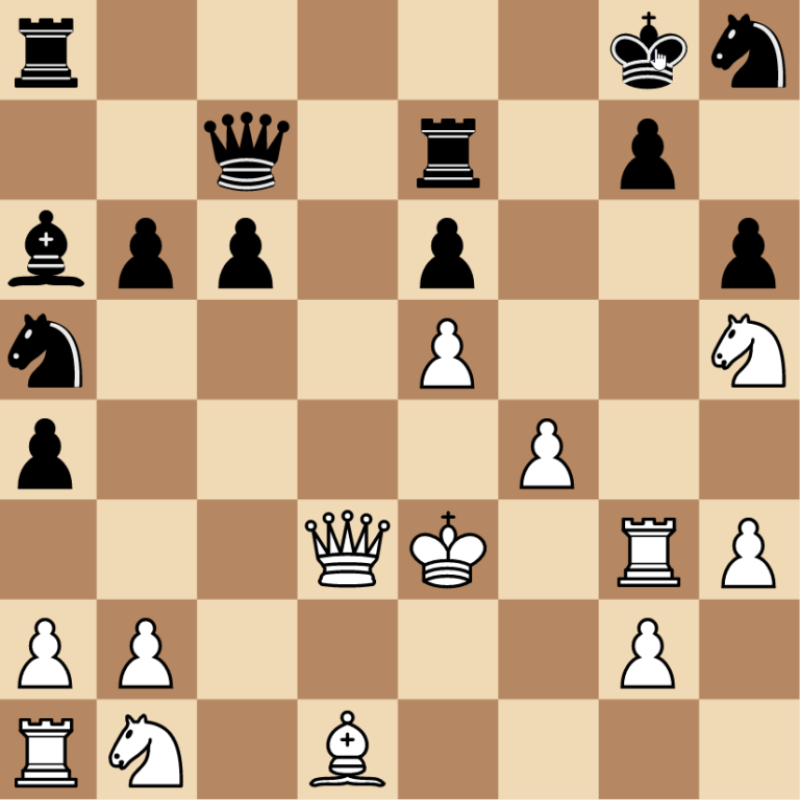
\includegraphics[width=0.25\linewidth]{./dataset/configLXIX.png}&
        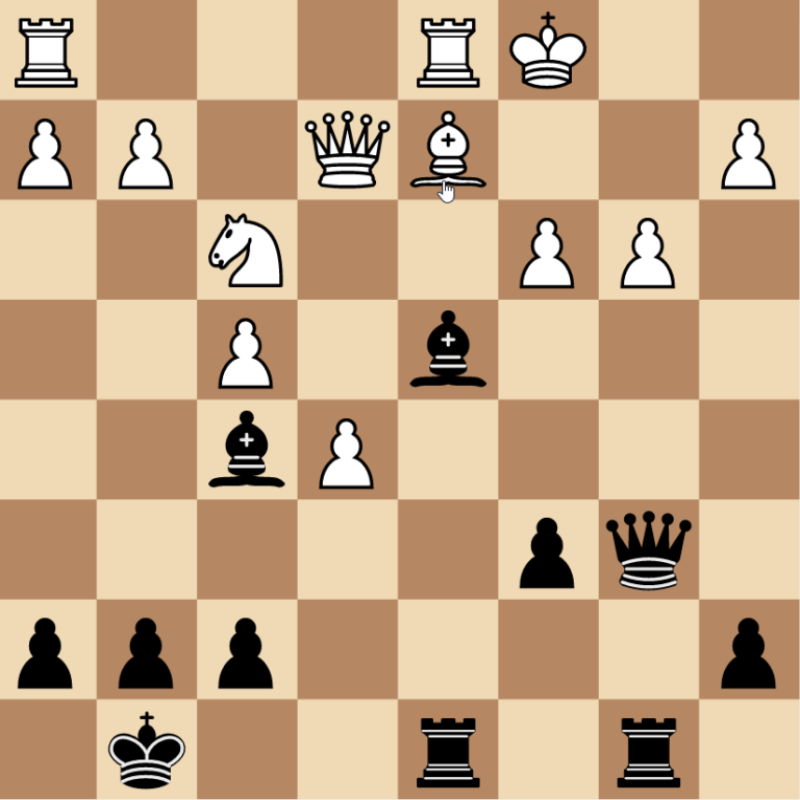
\includegraphics[width=0.25\linewidth]{./dataset/configLXVII.png}&
        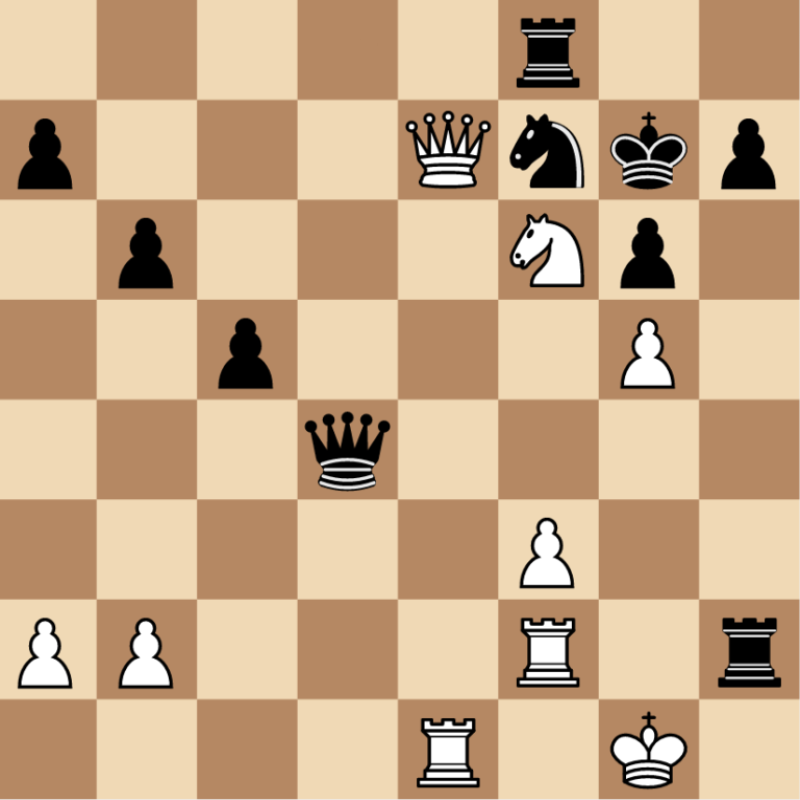
\includegraphics[width=0.25\linewidth]{./dataset/configRXLII.png}&
        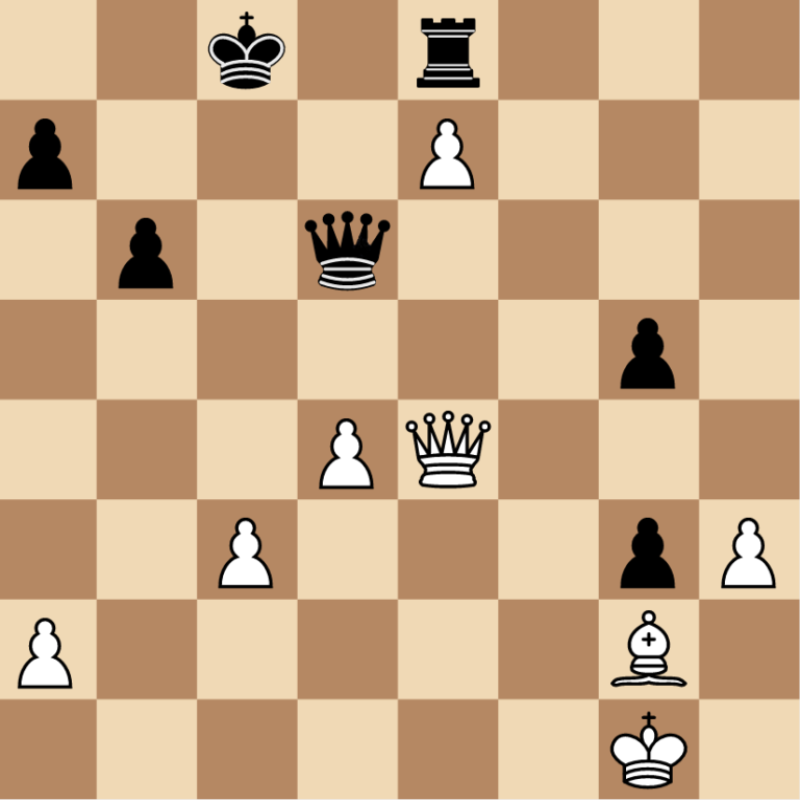
\includegraphics[width=0.25\linewidth]{./dataset/configV.png}\\
    \end{tabular}

     \begin{tabular}{@{}c@{\hspace{0.2cm}}c@{\hspace{0.2cm}}c@{}}
        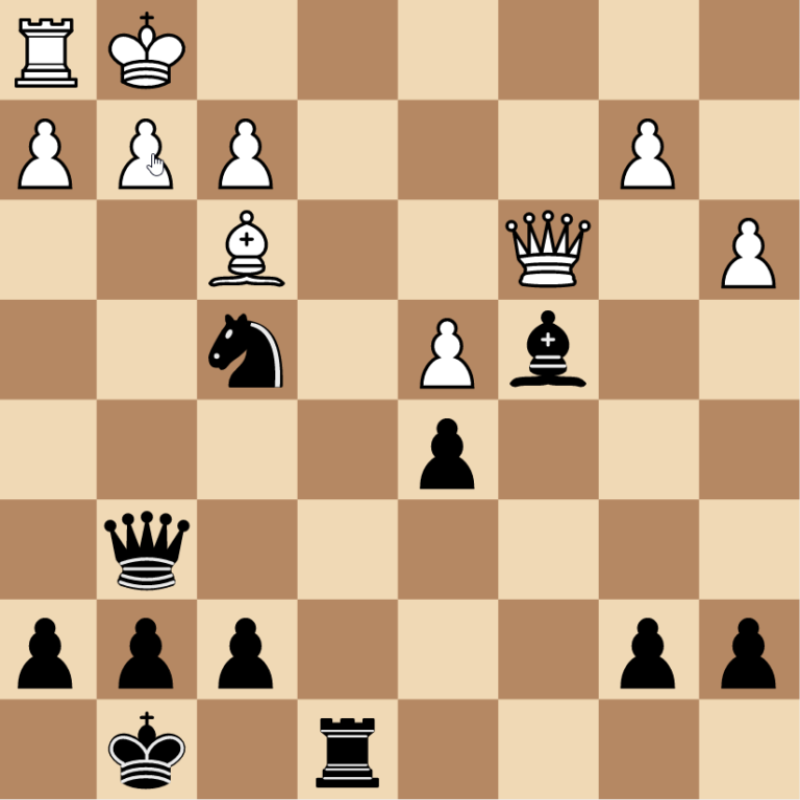
\includegraphics[width=0.25\linewidth]{./dataset/configXVI.png}&
        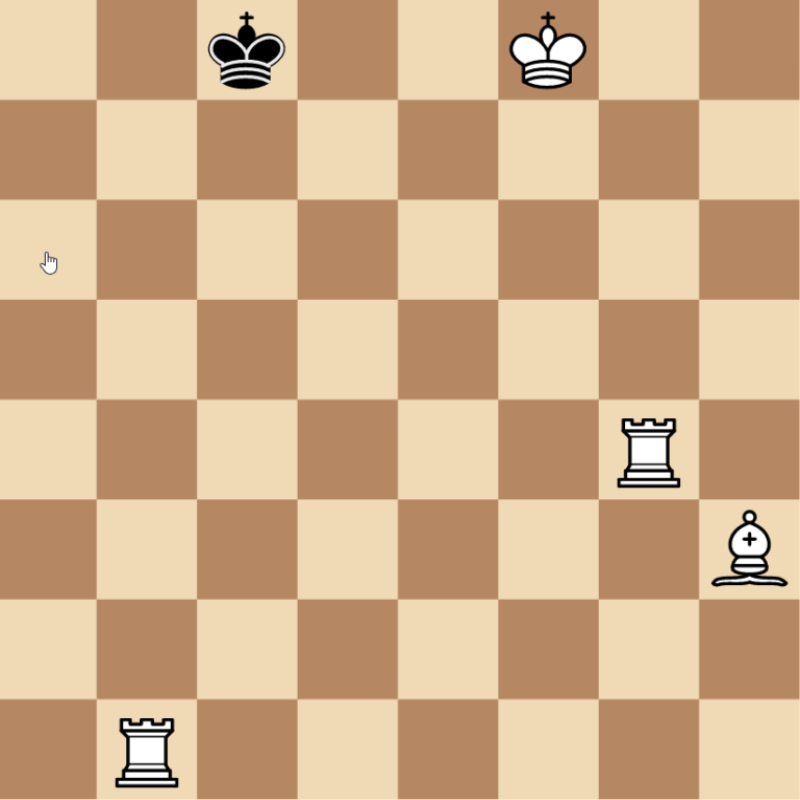
\includegraphics[width=0.25\linewidth]{./dataset/configXVII.png}&
        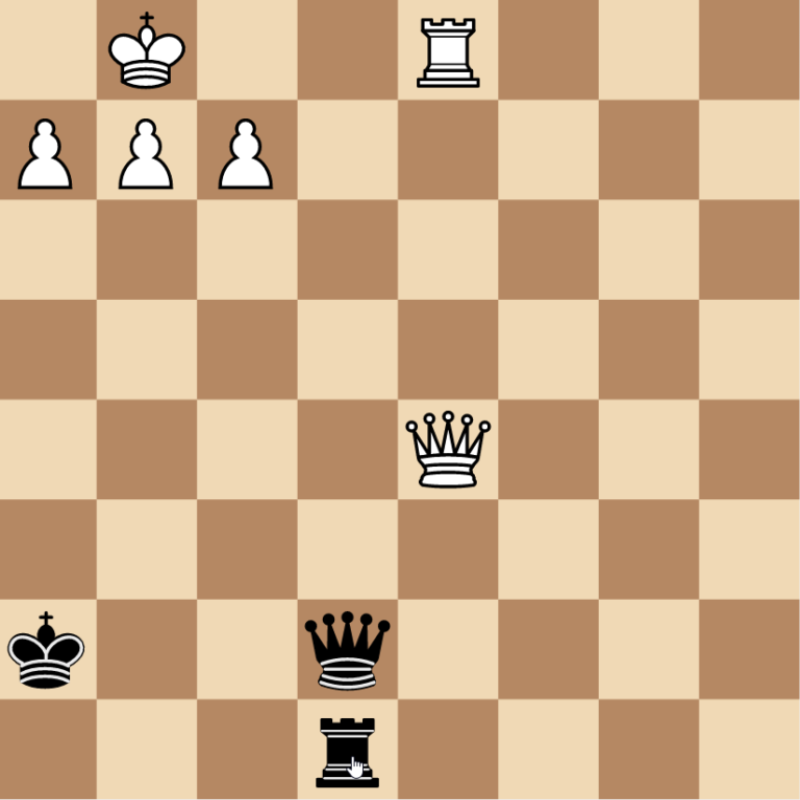
\includegraphics[width=0.25\linewidth]{./dataset/configXXIX.png}\\
       
    \end{tabular}
    \caption{Our dataset}
    \label{fig:dataset}
\end{figure}
    

Also as we mentioned when talking about Reingold  and al. work \cite{doi:10.1167/17.3.4,Charness2001}, "expert" players tend to look at the center of important configuration. When averaging players's eyetracking data we noticed than "expert" fixations were positioned on the most salient part of the saliency map, where most people were looking at, despite not being the most representative part of the players we had.

This little prepossessing done, we end up with 11 configurations and the same amount of saliency maps.
With such limited data, we needed ways to augment it while keeping data interesting and relevant.
\subsection{Data augmentation}
Data augmentation is the act creating variations of the dataset, to multiply the examples the network will learn on and help him generalize even more its knowledge to more and more complex examples. This include many transformation such as rotation, translation, flipping the image, scaling, cropping a part of the image , or even adding some noise to it to add some difficulty.

    \subsubsection{Cutting  board}
    The first augmentation we could think of was cutting the board into smaller pieces, same thing for the corresponding saliency map. So we could force the network to focus on specific parts of the board and learn how to look at those. We started with cutting it in four "4x4" part each being a quarter of the original board. We then thought about cutting in three by three  and five by five parts. But those being odd numbers of cell we needed to do the convolution of this cutting over the board on row and one column at a time. Doing that we had multiplied the amount of data by 150.
    \begin{figure}[ht!]
    \centering
    \begin{tabular}{@{}c@{\hspace{0.4cm}}c@{}}
        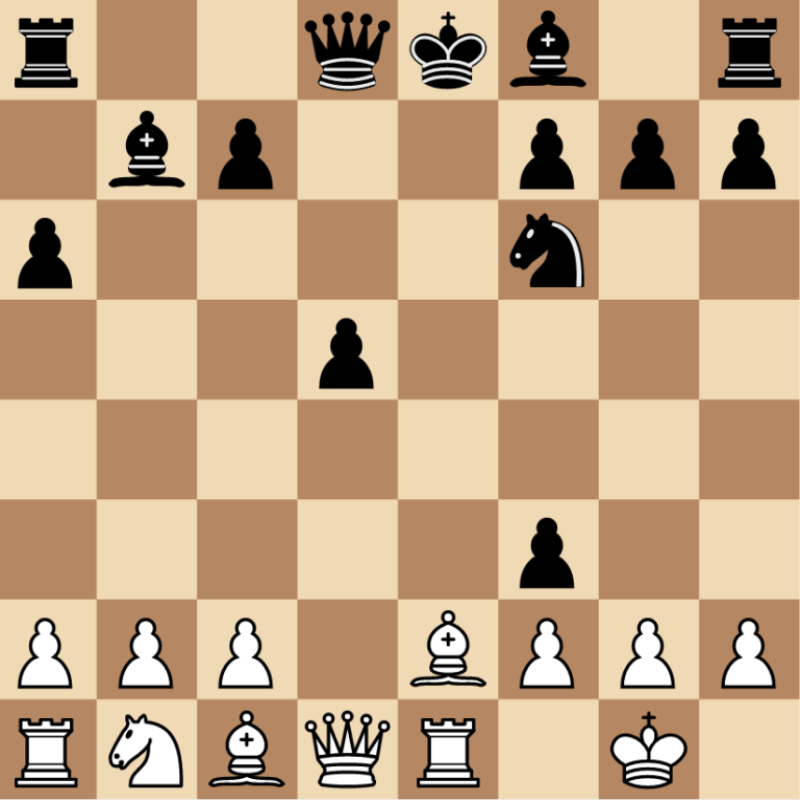
\includegraphics[width=0.25\linewidth]{./transformations/config.png}&
        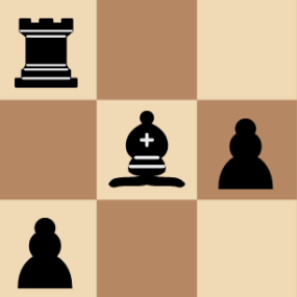
\includegraphics[width=0.25\linewidth]{./transformations/3.png}\\
        {\small  Configuration reference} & {\small Cutting in 3*3 cells}\\
         {\small  } & {\small }\\
        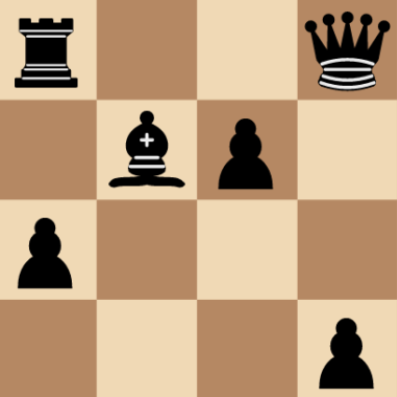
\includegraphics[width=0.25\linewidth]{./transformations/4.png}&
        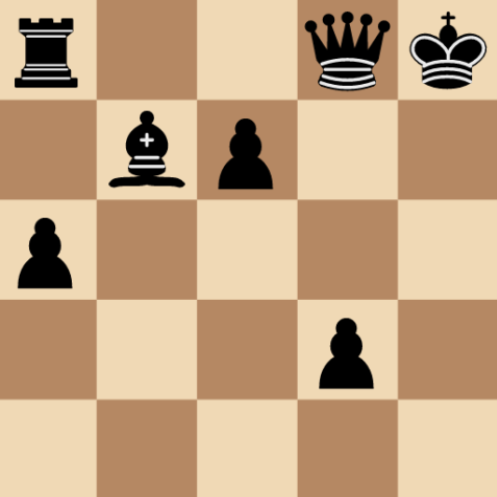
\includegraphics[width=0.25\linewidth]{./transformations/5.png}\\
        
        {\small  Cutting in 4*4 cells} & {\small Cutting in 5*5 cells} \\
         {\small  } & {\small }\\
    \end{tabular}
    \caption{Configuration and how it we cutted it}
    \label{fig:cutting}
\end{figure}
    
    \subsubsection{Pieces color inversion}
     An other augmentation was to invert the color of each piece (black to white and white to black). Because every configuration is possible while playing white and black, inverting colors was adding diversity of configurations the network could see. 
     To do that we used a neural network trained to classify chess pieces, we just needed to identify the cell color to replace the piece on each cells.
     \begin{figure}[ht!]
    \centering
    \begin{tabular}{@{}c@{\hspace{0.4cm}}c@{}}
        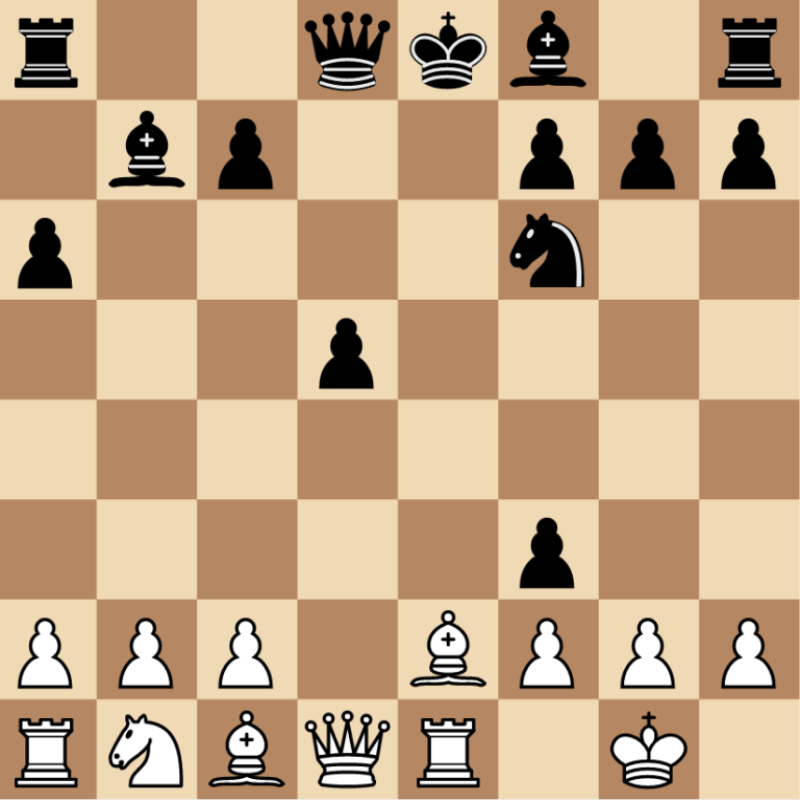
\includegraphics[width=0.25\linewidth]{./transformations/config.png}&
        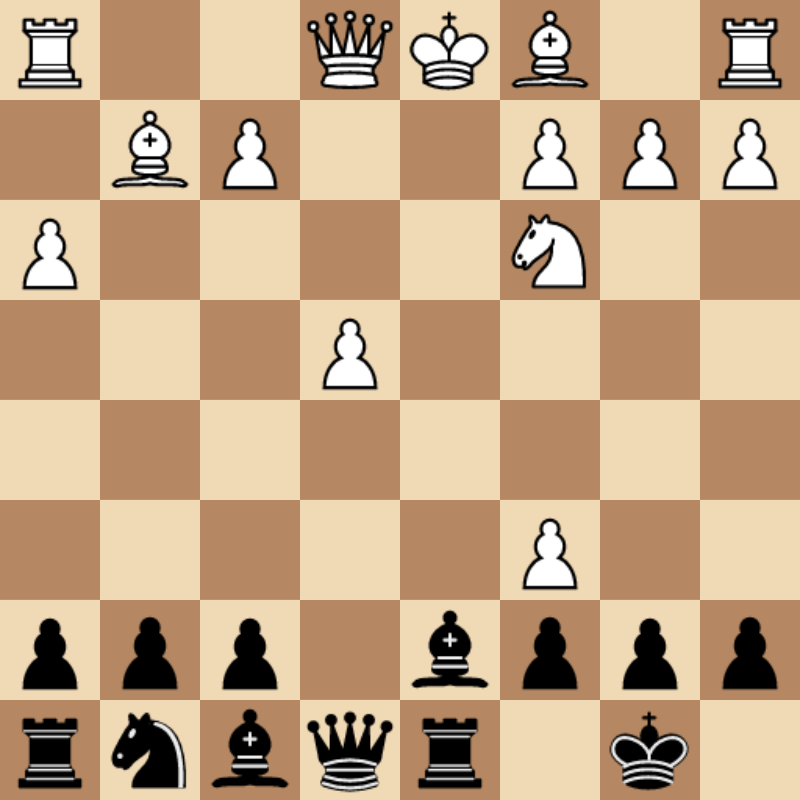
\includegraphics[width=0.25\linewidth]{./transformations/inverted.png}\\
       
        {\small Reference configuration} & {\small Same configurations } \\
        {\small} & {\small  inverting colors } \\
         {\small  } & {\small }\\
    \end{tabular}
    \caption{Configuration and its inverted counterpart}
    \label{fig:cutting}
\end{figure}
     
    \subsubsection{Flipping board}
    The last augmentation we used is  to change the orientation of the board, to the point of view of the other player. We considered that at any point of time, a chess player exploring his adversary possibilities would look at the board the same way he does. 
    
    \begin{figure}[ht!]
    \centering
    \begin{tabular}{@{}c@{\hspace{0.4cm}}c@{}}
        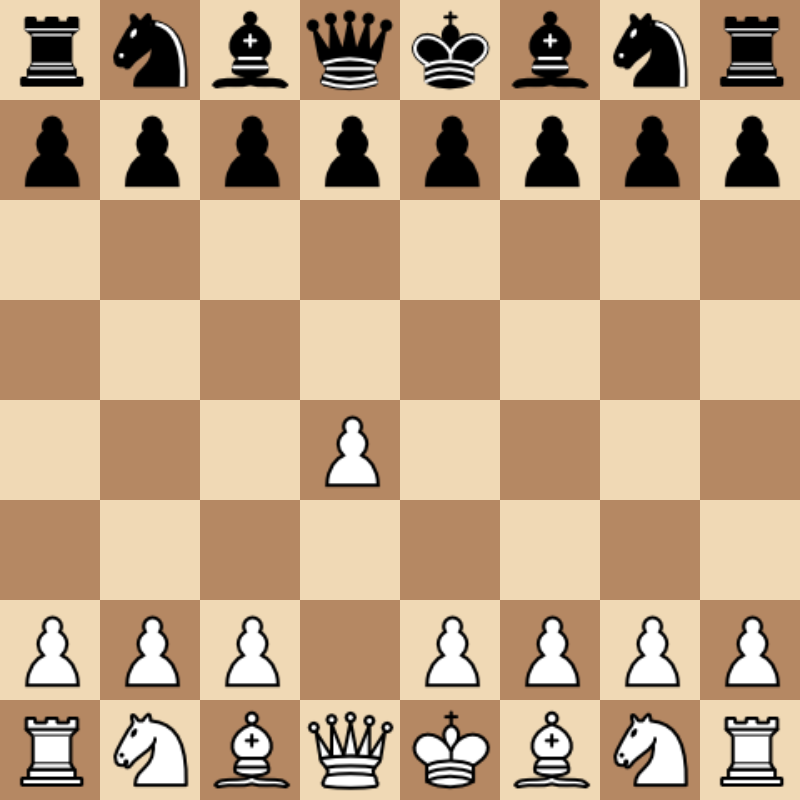
\includegraphics[width=0.25\linewidth]{./transformations/one_side.png}&
        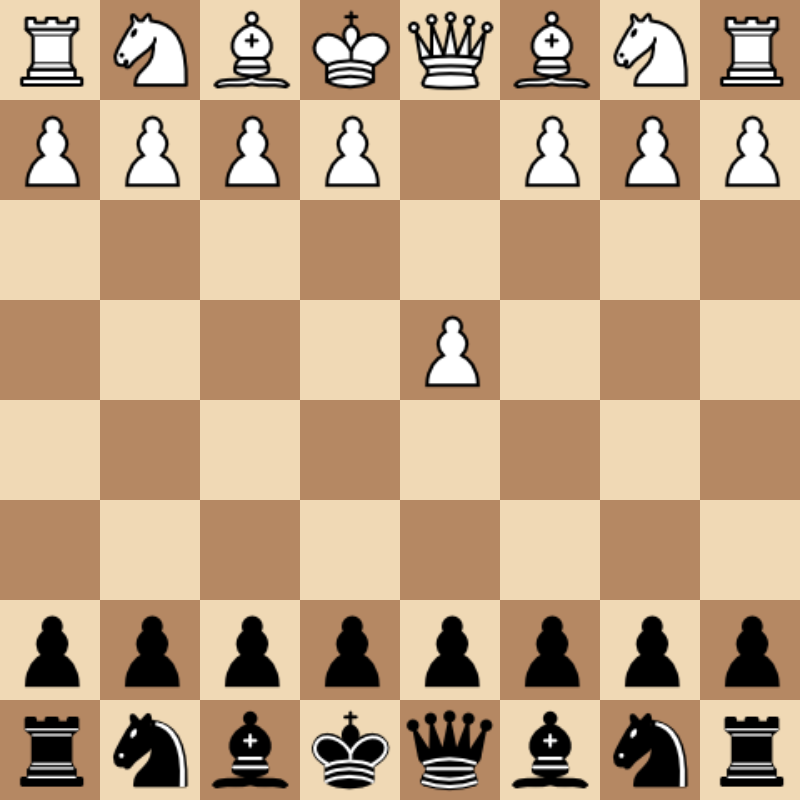
\includegraphics[width=0.25\linewidth]{./transformations/other_side.png}\\
       
        {\small Reference configuration} & {\small Same configurations  } \\
        {\small } & {\small  from enemy point of view} \\
         {\small  } & {\small }\\
    \end{tabular}
    \caption{Configuration and its inverted counterpart}
    \label{fig:cutting}
\end{figure}

\subsection{Training}

Training a deep neural network in an efficient way, as teaching a young child is not an easy and well defined process. Even though the algorithm is defined, its hyper parameters such as learning rate and how to set them, is very difficult and task dependant, requiring some prior thinking and attempts.  
For our problem we faced some difficulties concerning the learning rate and how to train using our data.


\subsubsection{Learning rate} 
Learning rate is one of the most important hyper-parameter when talking about training neural networks in an optimal way.
The bigger the learning rate is , the faster the weight will decrease toward a local minimum, but not necessarily to a good minimum.
That is why setting the learning rate to a value not too big to avoid some false minimum, but no too little to avoid too long training time. In his paper Leslie N. Smith \cite{DBLP:journals/corr/Smith15a} propose a cyclical learning rate, accelerating convergence toward a better accuracy than with a standard modification of learning rate. We use this strategy and compared it to the standard strategy of making the learning rate decrease after a certain amount of epochs. The learning rate was set at a maximum of 0.01 and a minimum of 0.0001.

\subsubsection{Using some prior training}

Even though the encoder part of our network is already trained and has his weights set for some features of Imagenet dataset \cite{imagenet_cvpr09}, the decoder part is at the beginning randomly initialized. The idea behind training our network on some other dataset before our own, is to initialize the decoder part to make it learn to transform features to salient or not part of the final saliency maps. 

Our first idea was to train it on the CAT2000 dataset \cite{DBLP:journals/corr/BorjiI15}, a dataset created by Borji and Itti, of about 4000 images for 20  different categories and 24 observers per images. The saliency maps of this dataset are created by convolving Gaussian of size  of 38px (size called degree of visual angle, DVA).

The second idea was to use the data created as described in then next section as this data would be more relevant to the chess problem.

\subsubsection{Training phases}

To avoid training a model for 10 days while it wasn't learning anything from the start, we made our training process as much explicit and easy to test as possible. Every 50 epochs a version of the model was saved and tested to visualize its progress. Loss was also monitored continuously. Various way of decreasing learning rate were tested. The main one which was considered as the most efficient was to train the network two thousands epochs at a time, and by looking at the loss for the last 100 epochs we decided or not to decrease the learning rate.

\section{Leading the network to learn tasks}

Top down approach in visual attention prediction is looking for relevant information in a picture depending on the task we have to accomplish. In chess the task is well defined as it is to move at a time T and for a specific configuration, the piece that is satisfying the most the condition which is : to win the game.
Because we are working with visual attention and saliency maps, we decided not to train a network to play chess (like Alphazero \cite{DBLP:journals/corr/abs-1712-01815}) and generate saliency maps depending on the pieces it considers to play at each round, but to create data leading the network to learn important pieces for a given configuration.

\subsection{Creating the data}
\subsubsection{Getting the configuration}
Since the beginning of the project we worked with Lichess \footnote{\url{https://en.lichess.org/} (last seen 06/2018)}. This online and offline chess platform allows to create personalized game and to play against other player or AI. With thousands of players registered and millions games played every month this is a gold mine to get data from. They even give access to a monthly database giving in the PGN format, all the games played during the past month. As an example for the month of March more than 22 million games have been played on this platform, giving us a quite big text file of 5 GB. Just with this file we would have enough data and nearly every used combinations in chess.

\subsubsection{From text to pictures}
From the beginning we have worked using screen capture of a chess game played on Lichess as an input for our network (the ground truth/target being a eye gazing heat map). So we needed to convert all the games we had to images to feed to our network.

PGN is a format giving for each turn the move done by white and black. Every move is based on the configuration of the board before the move and in the beginning black and white on their side of the board. Moves can be encoding as simple as two characters as "e4" for a pawn moving to e4 from e2. Or in a more complex way as "Nbxc3" for a knight moving from b2 and capturing a piece in c3. 
Without going into more details, what we needed to do was to create a parser to PGN format taking into account the complexity of the notation to create images from few lines of text. 

Once this done, we got from thousands of games, thousands of corresponding images.

\subsubsection{From a move to its heat map}

Because creating eye gazing data without an eye tracker is not really possible or would take a long time and wont be really objective, we needed to find a way to fake it while creating meaningful data. 
The idea we got was that a player when moving a piece looks at its destination and where it comes from. Even if it doesn't include the ultimate goal of a player when he is moving the piece (putting the enemy king in check or threatening a enemy's piece), it gives at least and idea on small areas and directions the player looks at.\\ 

\textbf{End and start points}\\

The first things we need to put as salient region are the start and end cells. We use for that a Gaussian shape a bit smaller than a cell, to represent a strong fixation.\\ 


\textbf{Trajectory}\\

From the origin and destination of a piece during each turn we would get two salient point, and adding the trajectory of the piece , we would get the path taken by the eye. This salient area is less bright than the end and start point as it doesn't correspond to long and strong fixations, but rather short and quick saccades. \\ 


\textbf{King in check}\\

We can also add the enemy king as a fixated point as when the move played is meant to put this king in check, we can consider that this piece is fixated by the player.\\ 

Figure \ref{fig:examplesconf} shows how a move can be transformed into a saliency map.

\begin{figure}[ht!]
    \centering
    \begin{tabular}{@{}c@{\hspace{0.1cm}}c@{\hspace{0.1cm}}c@{}}
        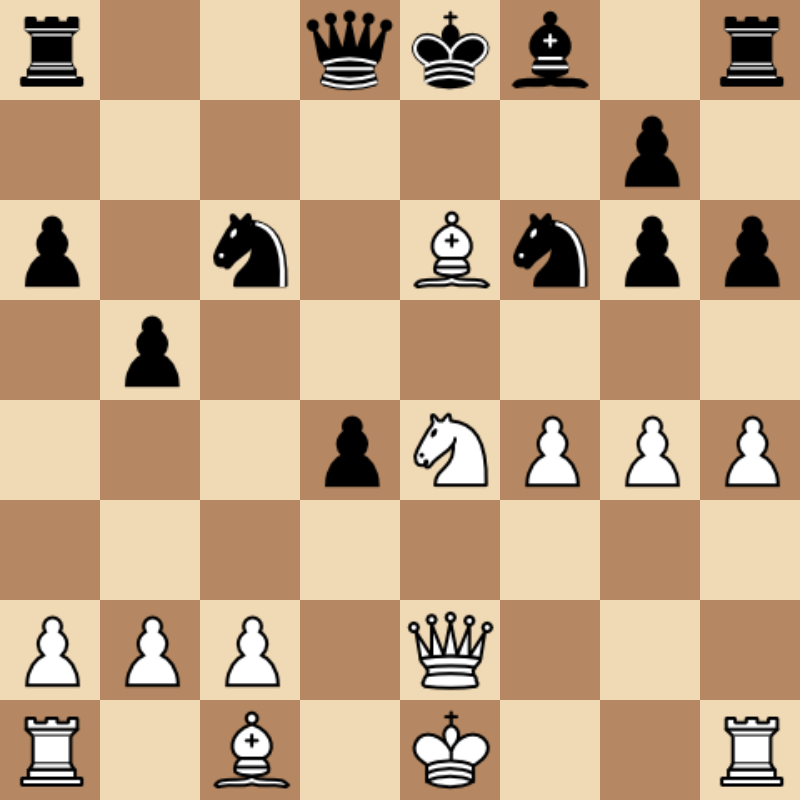
\includegraphics[width=0.25\linewidth]{./pics/config1.png}& 
        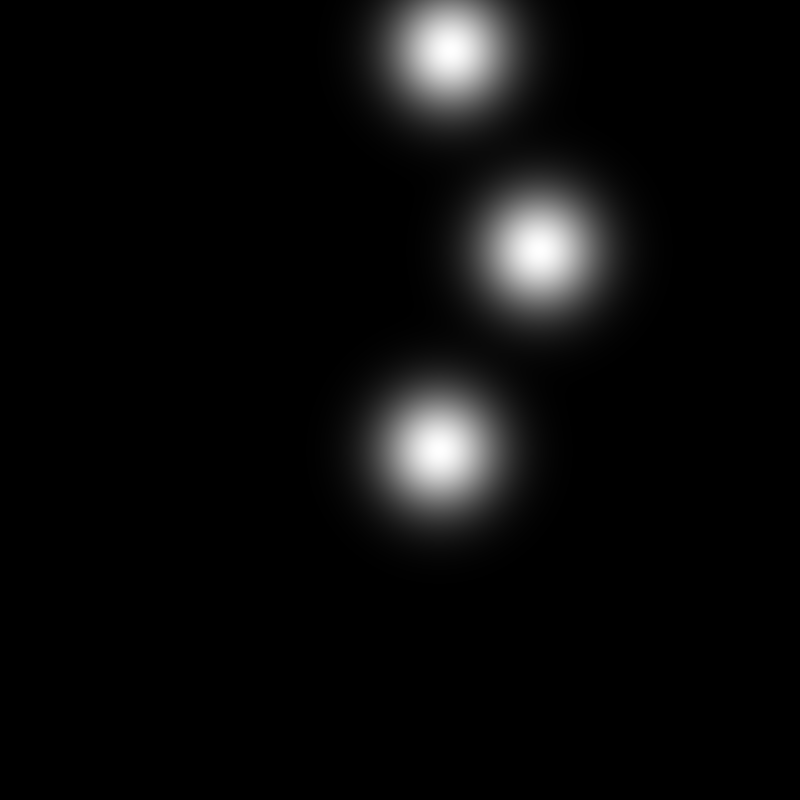
\includegraphics[width=0.25\linewidth]{./pics/saliency1.png}&
        
\includegraphics[width=0.25\linewidth]{./pics/bishopmove.png}\\
        
        {\small  Configuration reference} & {\small Salient points } & {\small The salient trajectory }\\
        {\small  Configuration reference} & {\small  (start, end, check)} & {\small  for a bishop}
    \end{tabular}
    \caption{Configuration and saliency map we can generate from it}
    \label{fig:examplesconf}
\end{figure}


\subsubsection{Final data}\label{section:descpnewdataset}

After all those steps we got a bigger dataset than what we were working with before. With around two thousands games and an average of fifty round each, giving us a bit more than one hundred and twenty thousands images that we can use as training data. Also this dataset was extensible as much as needed. Because we got our data from an opensource database containing Billions and Billions of games from thousands of players, the amount of data we could add to the dataset was quite huge. But we still limited the size of the dataset, to be able to train a minimum amount of epochs on it and because the generation of data, even in parallel was taking quite some time because of the disc operations when creating images.


Even though this new dataset was consequent and rich enough, some biases were still present.
The first one was that even with the large amount of configuration created, the vast majority of them were openings and their number being limited, there were a lot of redundancies.
The second bias was subjectivity of the saliency maps created. And the last one was the pieces moved compared to the number of pieces for each type. Pawns being the vast majority of them, they are often way more salient because they are  moved more often. Queen, rooks, knights and bishops follow pawns in the salient order. And the king being not very often moved and the center of attention as it is not put in check that often, had a limited saliency even for configuration where it was in danger.
Results of those bias are going to be illustrated in the Results chapter.

\subsection{From Saliency map to fixations}
Saliency map are continuous representation of visual attention. But in reality visual attention as captured by eye tracker is rather a set of fixations over the picture/screen. To get the fixations from a generated saliency map we used a local maxima computation algorithm. This algorithm is quite simple and consists on doing the convolution of a filter over the saliency map taking maximum for each convolution.
We chose to use a filter of the size of a cell, as we can consider that we fixate pieces or cells rather than their intersections. We also threshold the maximum values found as even if a value is a maximum compare to its surrounding it is not necessarily a fixation but rather a saccade. For this threshold we used values corresponding to the top 5,10 or 20\% of the whole map. To really see them we added a Gaussian shape of the size of a cell on them as seen in figure \ref{fig:fixat}

\begin{figure}[ht!]
    \centering
    \begin{tabular}{@{}c@{\hspace{0.1cm}}c@{\hspace{0.1cm}}c@{\hspace{0.1cm}}}
        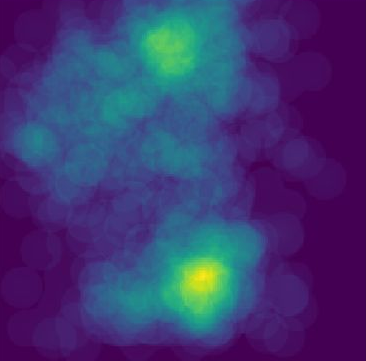
\includegraphics[width=0.30\linewidth]{./picsres/saliency_map_ori.png}& 
        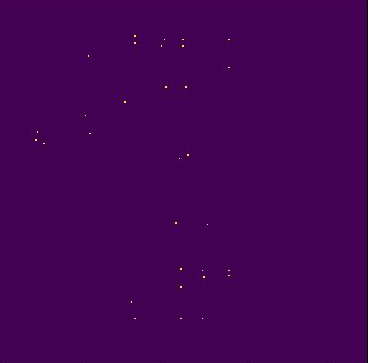
\includegraphics[width=0.30\linewidth]{./picsres/fixations_ori.png}& 
       
    
        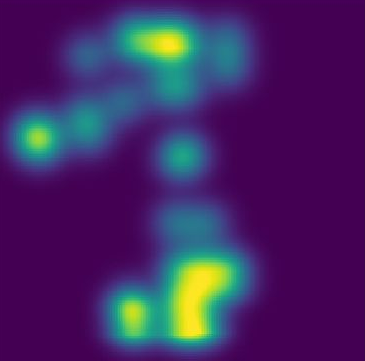
\includegraphics[width=0.30\linewidth]{./picsres/gaussians_ori.png}\\
       
         {\small Saliency Map} & {\small Fixations} & {\small Gaussian convoluted on fixations} \\
    \end{tabular}
    
    
    \caption{}
    \label{fig:fixat}
\end{figure}


\section{Implementation}

The deep learning part of the work have been implemented using the Python framework : Pytorch \cite{pytorch}. This framework offer a tensor based computation system with strong GPU acceleration. It also has a Deep Neural network building system, making the computations for the forward pass completely transparent and user made. This Framework is fast and powerful, completely suited for the work of designing a neural network and training it as we wanted.\\

All the prepossessing of data and its creation were made using python language and Numpy arrays. Same thing goes for the implementation of metrics and various code for loading data and organize training and testing. We didn't want to depend from too much libraries and limited their number to the strict minimum coding every algorithm ourselves in Python.\\

The computer we used for training and testing our network had a Nvidia 1080 as GPU, an Intel 40x Xeon E5-2630 and 132 GB of Ram available.

\subsection{Managing data in memory}
Memory space was not really a problem for us with the available space on the machine we use for training purposes. At least it was the case until we created our new dataset. With our augmented first dataset, we chose a simple but efficient way of loading the data directly in the 12GB V-RAM of our GPU. Doing so, for a small loading time we removed the transfer time between RAM and GPU, and increased the computing time during the training.
On the other hand we chose not to follow this strategy when training with our new dataset. As it is significantly bigger than the previous one it was impossible to load it all at one in the GPU memory. We chose to use the Pytorch's multi-workers functionality to ease and optimize the way our data was loaded in the GPU memory. This functionality creates threads in charge of loading batches into memory as they are needed by the training process.



